\documentclass[final]{beamer}
\mode<presentation> {
    \usetheme{I6dv}
}
\usepackage{amsmath,amsthm, amssymb, latexsym}
\usefonttheme[onlymath]{serif}
\usepackage[orientation=portrait,size=a1,scale=1.4,grid,debug]{beamerposter}                  % e.g. for DIN-A1 poster, with optional grid and debug output
\usepackage{graphicx}
\usepackage{epsfig}
\usepackage{xspace}
\usepackage{listings}
\usepackage{caption,subcaption}
\newcommand{\mm}{\mathrm}
\newcommand{\mb}{\mathbf}

\graphicspath{ {../../../presentations/lbnl_intro_sept13/figures/} }

\title[Abstract \#78]{New generation of LLRF and beam-based feedback stability models}
\author[C. Serrano, J. Byrd, L. R. Doolittle, G. Huang, A. Ratti, LBNL, D. Driver, A. Queiruga, UCB, Q. Llimona, UPF]{
    C. Serrano\inst{1}, J. Byrd\inst{1}, L. R. Doolittle\inst{1}, D. Driver\inst{2}, G. Huang\inst{1}, Q. Llimona\inst{3}, A. Queiruga\inst{2}, A. Ratti\inst{1}
}

\institute[shortinst]{
    \inst{1}%
    Lawrence Berkeley National Laboratory, Berkeley, CA 94720\\
    \inst{2}%
    Univesity of California, Berkeley, CA 94720\\
    \inst{3}%
    Universitat Pompeu Fabra, Barcelona, 08018, Spain
}


\date[Oct. 2013]{Oct. 2013}

\begin{document}
  \begin{frame}{}
    \begin{block}{Abstract}
    All RF groups in the accelerator community use modeling to some extent for LLRF development, and LBNL has traditionally invested a significant effort in this area for a number of reasons. It is possible to solve many
issues in the control algorithms in a comfortable software environment, often well before the availability of production systems. Software and hardware designs can be combined in simulation, easing the transition to final hardware system integration. Over time we have built a solid base of generic models which can be applied to a variety of machines and configuration schemes. The low-level implementation of the models has been re-implemented and extended to include elements in beam-based feedback loops and optimized to improve computation speed, memory usage, scalability and flexibility. The way they are configured and interact with high-level software has has been greatly improved to provide clean APIs and a convenient configuration scheme accessible from user-friendly tools such as GUIs and websites.
    \end{block}
		\begin{block}{User Interface}
		  \begin{columns}
		    \begin{column}{0.6\textwidth}
		      \begin{figure}
		      	\centering
			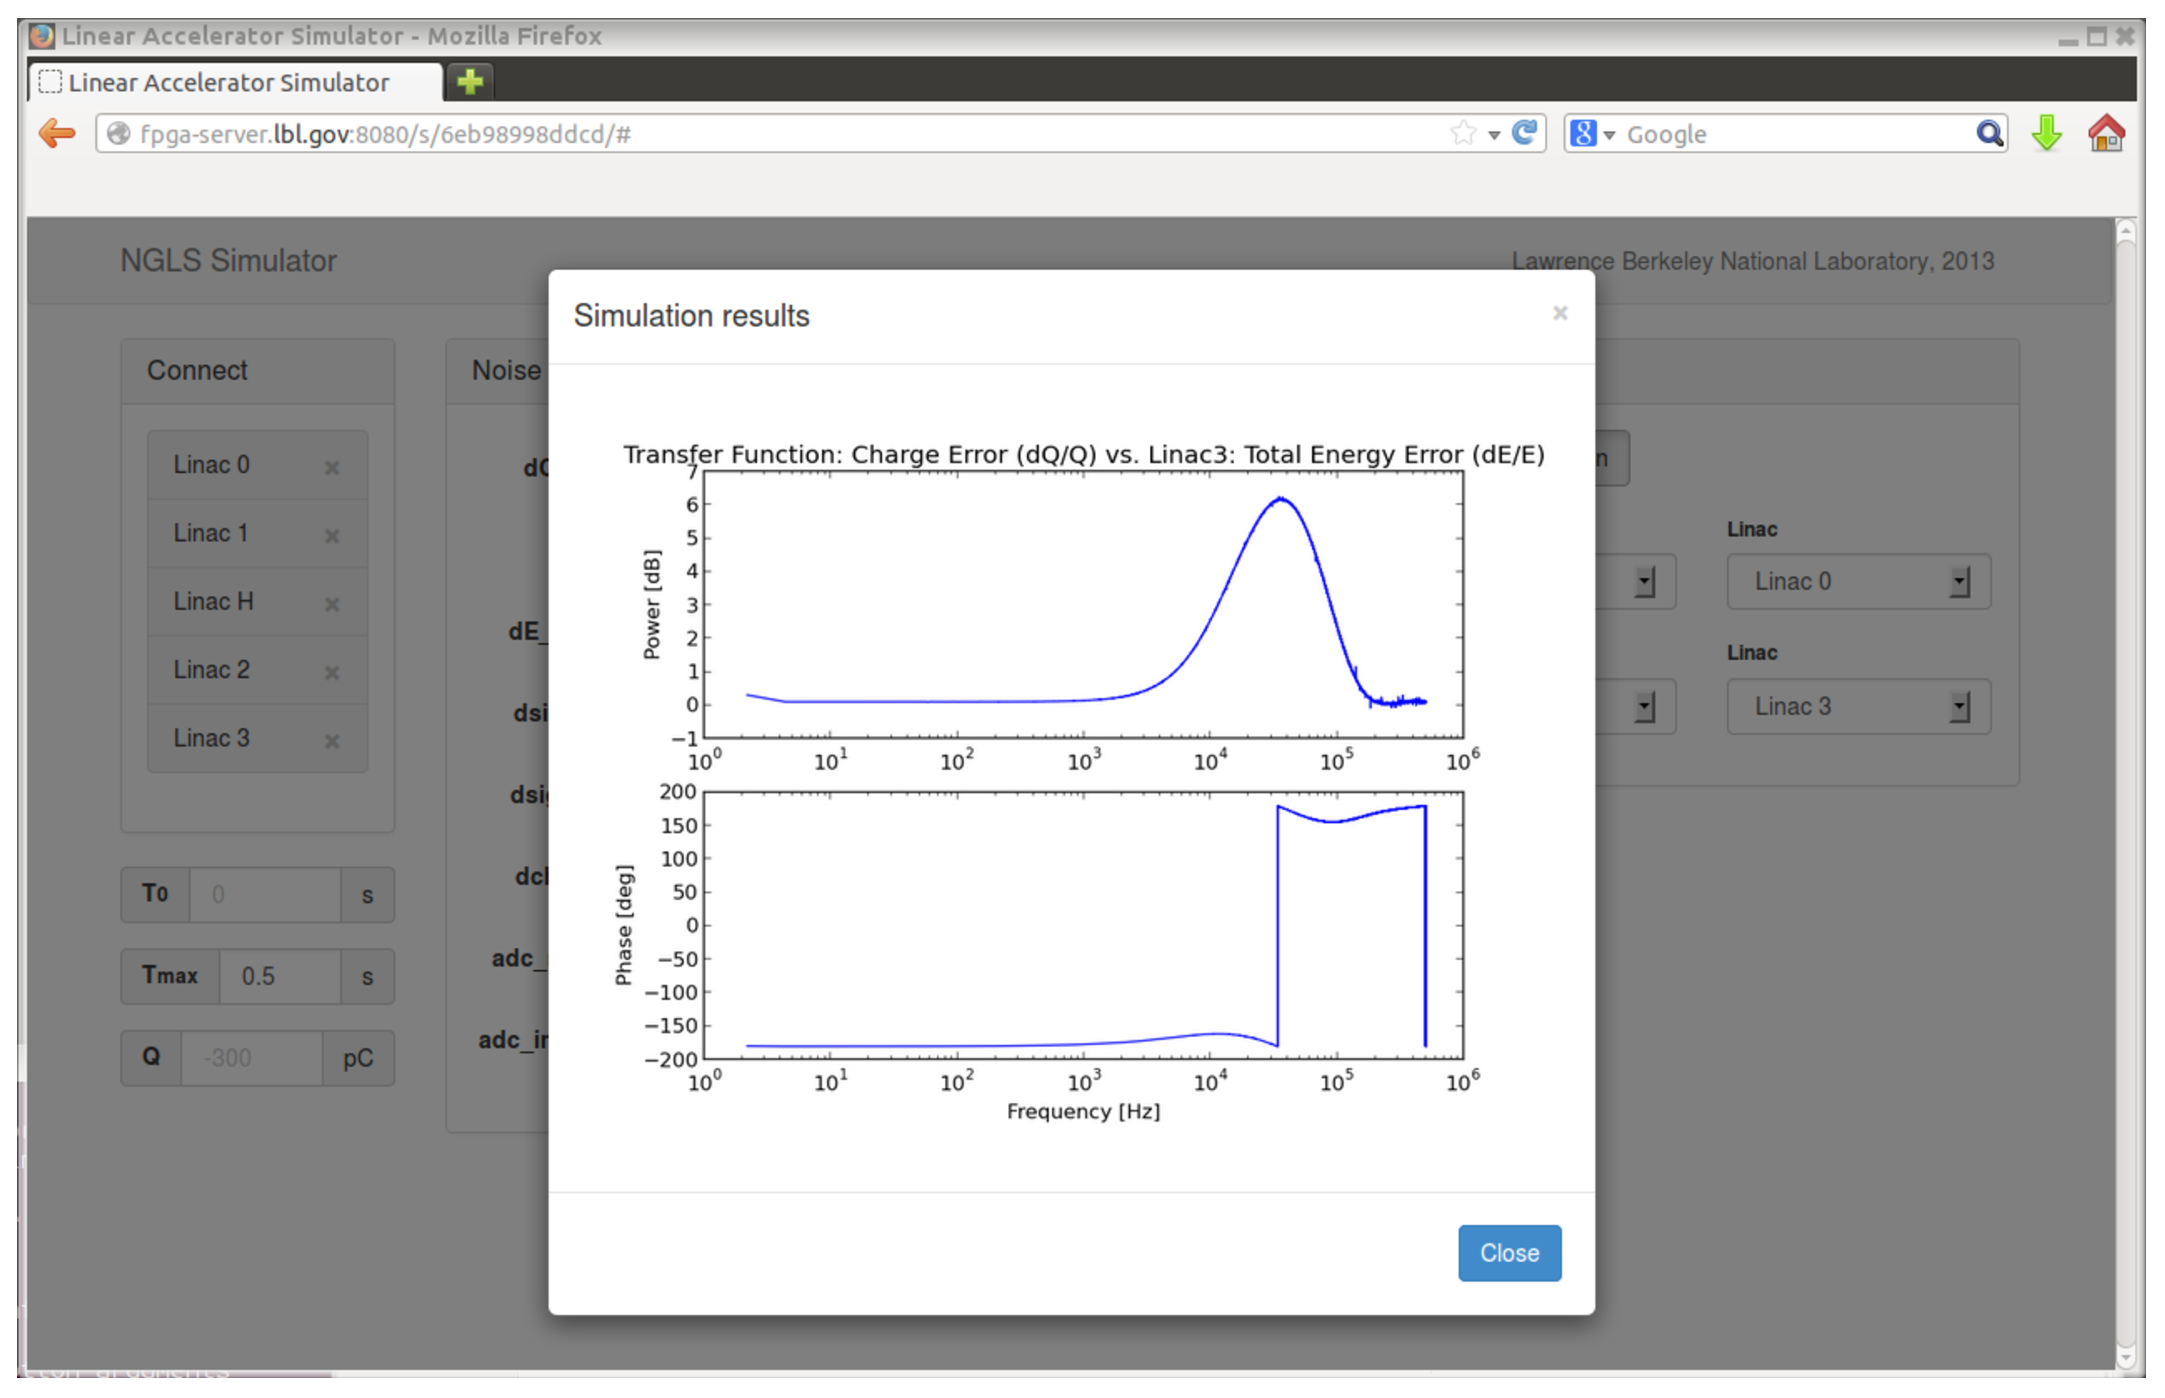
\includegraphics[width=\textwidth]{../figures/simulator_screenshot.eps}
		      \end{figure}
		    \end{column}
		    
		    \begin{column}{0.3\textwidth}
% 		      \begin{figure}
% 		      	\centering
% 			\includegraphics[scale=0.75]{architecture.eps}
% 		      \end{figure}
	          \begin{itemize}
	            \item Convenient, web-based user interface to mask back-end and configuration details.
		     \item JavaScript based,
		     \item Creates JSON configuration files from user input and runs the simulator back-end,
		     \item Handles configuration file, result and plot storage for easy retrieval,
		     \item Runs Hash on configuration file (including git commit ID) and skips running simulation if it has been run before.
		    \end{itemize}
		    \end{column}
		  \end{columns}
		\end{block}
    \begin{columns}[t]
      \begin{column}{.47\textwidth}
        \begin{block}{Simulation data flow}
	\begin{figure}
	  \centering
	  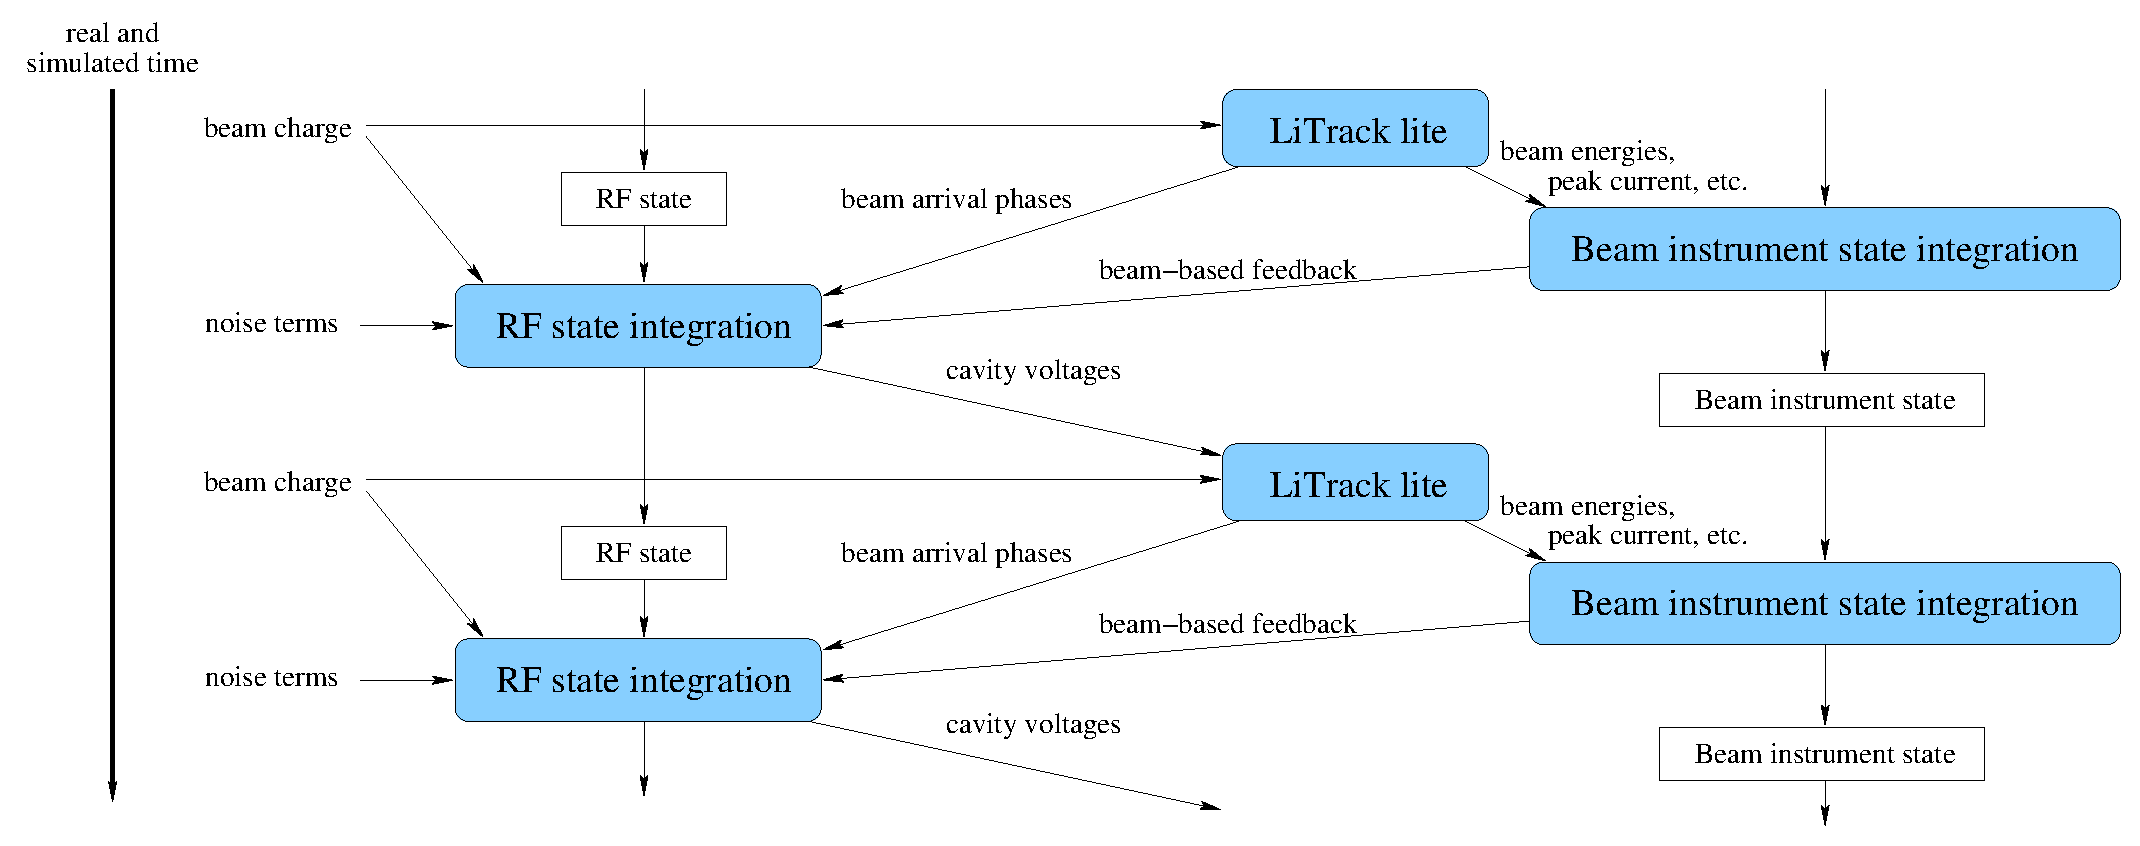
\includegraphics[width=\textwidth]{model_do2.eps}
	\end{figure}
	\begin{itemize}
	 \item Integrated particle longitudinal tracking simulator with LLRF and beam-based feedback models,
	 \item Full integration of instrumentation models, along with LLRF controller and different noise sources,
	 \item Any part of the system can be enabled/disabled and configured to match any Linac configuration.
	\end{itemize}


        \end{block}
      \end{column}
      \begin{column}{.47\textwidth}
        \begin{block}{Simulation engine architecture}
	    \begin{column}{0.35\textwidth}
	      \begin{figure}
		\centering
		\includegraphics[width=\textwidth]{architecture.eps}
	      \end{figure}		    
	    \end{column}
	   \begin{column}{0.6\textwidth}
	      \begin{figure}
		\centering
		\includegraphics[width=\textwidth]{shallowoutline.eps}
	      \end{figure}		    
	    \end{column}
	\begin{itemize}
	\vspace{1cm}
	 \item High-performance: 30 seconds for 1.2M steps,
	 \item Documented, unit tests, and Python interface.
	\end{itemize}

        \end{block}
        
      \end{column}
    \end{columns}
  \end{frame}
\end{document}
